\documentclass[
	a4paper,
	10pt,
	unnumberedsections,
	twoside,
]{LTJournalArticle}

\addbibresource{referencias.bib}

\usepackage[utf8]{inputenc}
\usepackage[T1]{fontenc}
\usepackage[spanish]{babel}
\usepackage{url}
\usepackage{booktabs}

\runninghead{Violencia interpersonal registrada en Colombia}

\setcounter{page}{1}

\title{Patrones de violencia interpersonal registrada en Colombia (2015--2024): preprocesamiento reproducible, cubo OLAP y dashboard anal\'itico}

\author{%
	Yeimy Vanessa L\'opez Terreros\thanks{C\'odigo: 1600047.} \and
	Javic Camilo Rojas Hurtado\thanks{C\'odigo: 1600047.} \and
	Juan Gonzales Mosquera\thanks{C\'odigo: 1600047.}
}

\date{\footnotesize Universidad de Los Llanos, Villavicencio, Meta, Colombia}

\renewcommand{\maketitlehookd}{%
	\begin{abstract}
		\noindent
		Se analizaron 981.611 casos de violencia interpersonal consignados por el Instituto Nacional de Medicina Legal y Ciencias Forenses (INMLCF) entre 2015 y 2024, a partir del conjunto \emph{Violencia interpersonal. Colombia, a\~{n}os 2015 a 2024. Cifras definitivas} en Datos Abiertos Colombia \cite{medicinalegal2024}.
		El trabajo aplic\'o CRISP-DM \cite{wirth2000crisp}: limpieza documentada en \texttt{src/prepare.py}, agregaciones OLAP offline y un dashboard Streamlit \cite{streamlit2024} organizado en cuatro ejes anal\'iticos.
		La serie anual alcanz\'o su m\'aximo en 2015 (126.803 casos) y su m\'inimo en 2020 (58.512); Bogot\'a D.C., Antioquia y Cundinamarca concentraron el 43{,}3\,\% de los registros; las v\'ictimas documentadas fueron en su mayor\'ia hombres (66{,}1\,\%) en edades j\'ovenes-adultas; tras homologar escenarios, \emph{V\'ia p\'ublica o calle} agrup\'o el 53{,}3\,\% de los casos.
		Los resultados describen patrones de \emph{registro administrativo}, no prevalencia poblacional.
	\end{abstract}
}

\begin{document}

\maketitle

\section{Introducci\'on}

La violencia interpersonal ---agresiones entre personas fuera del marco estrictamente intrafamiliar de pareja--- genera lesiones, incapacidades y costos sociales en Colombia.
Una parte de esos hechos accede a valoraci\'on medicolegal y queda registrada en bases administrativas abiertas del INMLCF \cite{medicinalegal2024}.
Esos registros ofrecen volumen, desagregaci\'on territorial y variables demogr\'aficas y situacionales, pero combinan ocurrencia del hecho, denuncia, derivaci\'on institucional y capacidad de captura; no deben leerse como censo de la violencia en la poblaci\'on.

CRISP-DM \cite{wirth2000crisp} ordena proyectos de anal\'itica desde la comprensi\'on del problema hasta el despliegue de resultados.
Este estudio documenta ese ciclo sobre datos abiertos del INMLCF, con separaci\'on expl\'icita entre procesamiento offline (dataset y agregados) e interfaz interactiva (dashboard), de modo que la sustentaci\'on y la consulta reutilicen la misma base procesada.

\textbf{Pregunta de investigaci\'on.}
\emph{¿C\'omo han evolucionado y qu\'e patrones temporales, territoriales y victimol\'ogicos caracterizan los casos de violencia interpersonal registrados en Colombia entre 2015 y 2024?}

\textbf{Objetivo general.}
Caracterizar esos patrones mediante un pipeline reproducible y comunicarlos en un dashboard de cuatro ejes anal\'iticos.

\textbf{Objetivos espec\'ificos.}
\begin{enumerate}
	\item Describir la din\'amica temporal del volumen registrado.
	\item Analizar la distribuci\'on territorial (departamento, municipio o localidad, zona urbana--rural).
	\item Caracterizar el perfil de v\'ictimas y la concentraci\'on por d\'ia y franja horaria.
	\item Examinar escenario, mecanismo de lesi\'on, severidad medicolegal y presunto agresor.
\end{enumerate}

\section{Metodolog\'ia}

\subsection{Fuente de datos}

El insumo proviene del portal Datos Abiertos Colombia, dataset \emph{Violencia interpersonal. Colombia, a\~{n}os 2015 a 2024. Cifras definitivas}, publicado por el INMLCF \cite{medicinalegal2024}.
La URL de consulta y descarga es \url{https://www.datos.gov.co/en/Justicia-y-Derecho/Violencia-interpersonal-Colombia-a-os-2015-a-2024-/e3xi-4zq5/about_data}.
El cat\'alogo reporta cerca de 982.000 filas y 35 columnas sobre lesiones no fatales por violencia interpersonal con valoraci\'on medicolegal.

Tras el pipeline descrito en las subsecciones siguientes, el universo anal\'itico qued\'o en \textbf{981.611 registros} (2015--2024) y \textbf{38 variables} en \texttt{data/processed/dataset.parquet}.
Toda cifra posterior se refiere a casos \emph{registrados}, salvo indicaci\'on contraria.

\subsection{Perfil de calidad inicial}

Antes del preprocesamiento se verific\'o:
\begin{itemize}
	\item cobertura temporal completa 2015--2024;
	\item ausencia de duplicados por identificador \texttt{id};
	\item la columna \texttt{contexto\_hecho} con una sola categor\'ia en el 100\,\% de filas del CSV (\emph{1 Lesiones no Fatales por Violencia Interpersonal}), sin variaci\'on anal\'itica;
	\item variantes ortogr\'aficas y taxon\'omicas en escenario, circunstancia y presunto agresor, propias de la codificaci\'on INMLCF y de exportaciones sucesivas.
\end{itemize}

\subsection{Preprocesamiento (\texttt{src/prepare.py})}

La limpieza se implement\'o en Python con reglas de dominio centralizadas en \texttt{app/text\_es.py}.
La Tabla~\ref{tab:prep} resume las etapas y su justificaci\'on; omitir cualquiera de ellas distorsiona agregados territoriales, perfiles demogr\'aficos o rankings de escenario y agresor.

\begin{table}[htbp]
	\centering
	\small
	\caption{Etapas del preprocesamiento y motivo anal\'itico}
	\label{tab:prep}
	\begin{tabular}{@{}p{0.22\linewidth}p{0.68\linewidth}@{}}
		\toprule
		\textbf{Etapa} & \textbf{Motivo} \\
		\midrule
		Lectura CSV con detecci\'on de encoding (\texttt{utf-8-sig}, \texttt{utf-8}, \texttt{cp1252}, \texttt{latin-1}) & Evitar p\'erdida de tildes y caracteres especiales antes de cualquier conteo \\
		Renombrado posicional a \texttt{snake\_case} & Contrato estable entre CSV fuente y c\'odigo \\
		Normalizaci\'on Unicode NFC y alias sem\'anticos (\texttt{DOMAIN\_ALIASES}) & Unificar etiquetas INMLCF equivalentes sin alterar categor\'ias distintas \\
		Estandarizaci\'on de faltantes (\texttt{MISSING\_PATTERNS} $\rightarrow$ \emph{Sin informacion}) & Comparabilidad entre variables categ\'oricas \\
		Normalizaci\'on de franjas horarias (\texttt{normalizar\_franja}) & Corregir espacios dobles en \texttt{rango\_hora} que fragmentaban el heatmap \\
		Canonizaci\'on modal (\texttt{canonize\_column}) en departamento, municipio, escenario, agresor, mecanismo, zona y circunstancia & Reducir duplicados por may\'usculas o tildes conservando la forma m\'as frecuente \\
		Derivadas \texttt{dias\_incapacidad\_num}, \texttt{severidad\_categoria}, \texttt{anio\_mes}, \texttt{fin\_semana} & Severidad ordinal y apoyo temporal sin releer el CSV \\
		Filtro temporal 2015--2024 & Alinear universo con el t\'itulo del dataset \\
		Exclusi\'on de \texttt{contexto\_hecho} del parquet exportado & Variable constante; no aporta a comparaciones \\
		\bottomrule
	\end{tabular}
\end{table}

\textbf{Homologaciones aplicadas} (decisi\'on documentada, no exhaustiva sobre toda la taxonom\'ia INMLCF):
\begin{enumerate}
	\item \textbf{Escenario:} tres etiquetas de v\'ia p\'ublica/calle (\emph{V\'ia P\'ublica}, \emph{Calle (autopista, avenida, dentro de la ciudad)} y variante CSV antigua) $\rightarrow$ \emph{V\'ia p\'ublica o calle} (523.085 casos, 53{,}3\,\%).
	\item \textbf{Circunstancia detallada:} cuatro pares duplicados solo por capitalizaci\'on o tildes; resueltos por frecuencia modal.
	\item \textbf{Presunto agresor:} \emph{Amigo (a)} y \emph{Amigo(a)} unificados en \emph{Amigo(a)}.
\end{enumerate}
Deliberadamente \emph{no} se fusionaron categor\'ias sem\'anticamente distintas del INMLCF (p.\ ej.\ \emph{Conocido} frente a \emph{Otros conocidos}), ni variantes adicionales de escenario como \emph{V\'ia p\'ublica} sin \emph{o calle}.

\subsection{Cubo OLAP y agregados (\texttt{analysis/run.py})}

El dashboard no carga las $\sim$980.000 filas en memoria.
\texttt{analysis/run.py} ejecuta \texttt{prepare()}, exporta el dataset limpio y genera cinco tablas Parquet en \texttt{data/processed/}:

\begin{itemize}
	\item \texttt{agg\_filtros.parquet}: hecho \texttt{casos}; dimensiones \texttt{anio\_hecho}, \texttt{departamento\_hecho}, \texttt{municipio\_hecho}, \texttt{sexo\_victima}, \texttt{zona\_hecho}, \texttt{pertenencia\_etnica}, \texttt{ciclo\_vital}.
	\item \texttt{agg\_territorial.parquet}: desglose departamento--municipio--localidad (localidad relevante para Bogot\'a D.C.).
	\item \texttt{agg\_demografia.parquet}: sexo, grupo etario quinquenal, ciclo vital.
	\item \texttt{agg\_patrones.parquet}: escenario, mecanismo, severidad y presunto agresor (columna \texttt{tipo}).
	\item \texttt{agg\_dia\_hora.parquet}: d\'ia de la semana y franja horaria.
\end{itemize}

El m\'odulo \texttt{app/analytics.py} filtra esas tablas con \texttt{FilterState} y suma el hecho \texttt{casos}; \texttt{app/filters.py} expone los selectores en el panel lateral.
Como exploraci\'on complementaria ---no visible en el dashboard--- se ejecut\'o K-means ($k=4$) sobre una muestra de 50.000 registros y ocho variables categ\'oricas \cite{pedregosa2011sklearn}.

\subsection{Dashboard Streamlit}

La aplicaci\'on (\texttt{app/streamlit\_app.py} y \texttt{app/pages/}) consume \'unicamente los agregados OLAP.
La arquitectura separa: \texttt{data\_loader.py} (carga Parquet), \texttt{analytics.py} (cortes), \texttt{charts.py} (Plotly), \texttt{narrative.py} (KPIs y textos por eje), \texttt{nav.py} (barra de secciones) y \texttt{kpi.py} (tarjetas de indicadores).

\textbf{Filtros globales} (sidebar, aplican a todas las vistas): periodo, departamento, municipio o ciudad, zona del hecho, sexo de la v\'ictima, pertenencia \'etnica y ciclo vital.

\textbf{Cuatro secciones} alineadas con los objetivos espec\'ificos:

\begin{enumerate}
	\item \textbf{Panorama} --- \emph{Casos registrados por a\~{n}o}: KPIs de periodo, l\'inea anual y lectura a\~{n}o a a\~{n}o.
	\item \textbf{Territorio} --- \emph{Casos por departamento y municipio}: ranking departamental, proporci\'on urbana--rural, drill de top 5 municipios o top 5 localidades en Bogot\'a D.C.
	\item \textbf{Personas y tiempo} --- \emph{Perfil de v\'ictimas y momento del hecho}: barras sexo--edad, ciclo vital por sexo (apilado en modo \emph{Ambos}), heatmap d\'ia--hora y top de franjas.
	\item \textbf{Patrones} --- \emph{Mecanismo, escenario, gravedad y agresor}: mecanismos y escenarios m\'as frecuentes, severidad medicolegal y presunto agresor en panel doble.
\end{enumerate}

Las figuras est\'aticas de este informe (\texttt{articulo/figuras/}) se generan en el mismo \texttt{run.py} con matplotlib a partir del dataset procesado.

\subsection{Herramientas}

Python 3.10+, pandas, numpy, PyArrow, scikit-learn, matplotlib, Plotly y Streamlit.

\section{Resultados}

\subsection{Din\'amica temporal}

La Figura~\ref{fig:anual} muestra la serie 2015--2024.
El m\'aximo corresponde a 2015 (126.803 casos); entre 2016 y 2019 los conteos permanecen por encima de 110.000.
En 2020 se registra el m\'inimo (58.512), seguido de recuperaci\'on parcial hasta 92.824 en 2023 y 82.809 en 2024.

\begin{figure}[htbp]
	\centering
	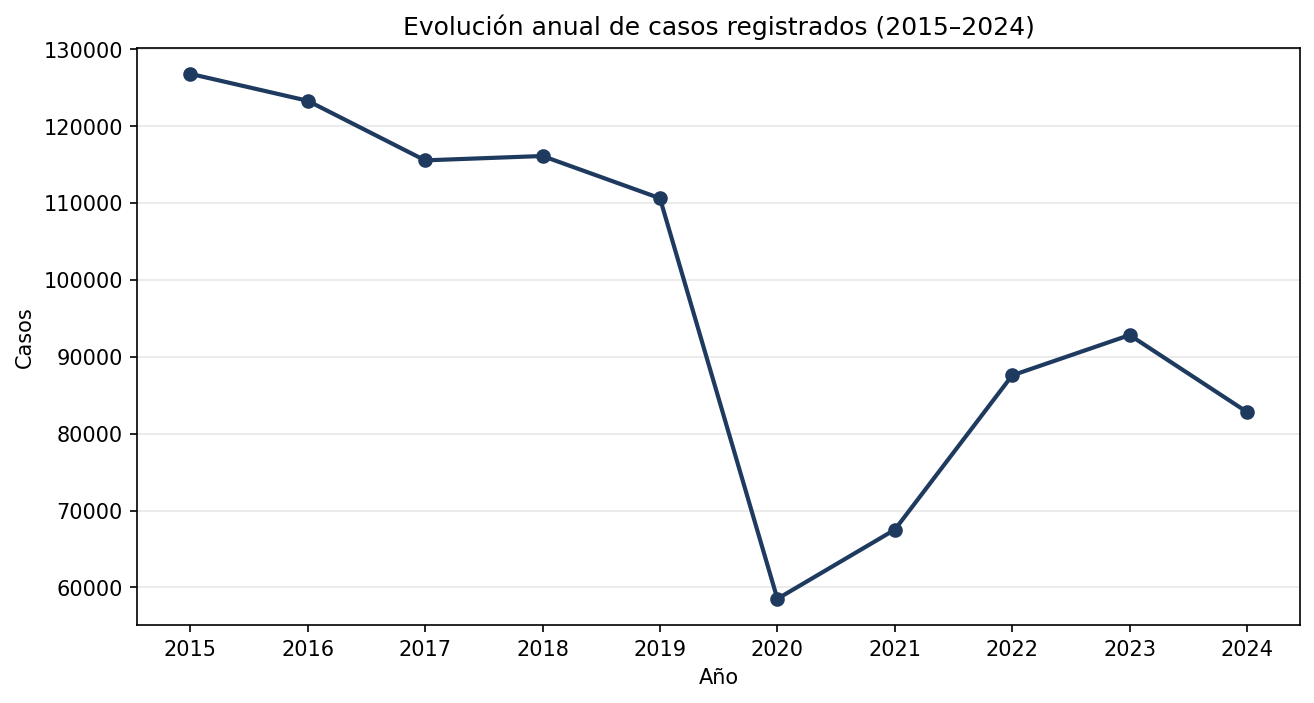
\includegraphics[width=0.92\linewidth]{figuras/01_evolucion_anual.png}
	\caption{Casos registrados por a\~{n}o. Elaboraci\'on propia con datos INMLCF \cite{medicinalegal2024}.}
	\label{fig:anual}
\end{figure}

\subsection{Distribuci\'on territorial}

Bogot\'a D.C. (239.220; 24{,}4\,\%), Antioquia (104.045; 10{,}6\,\%) y Cundinamarca (81.221; 8{,}3\,\%) encabezan el ranking (Figura~\ref{fig:dept}).
Los cinco primeros departamentos suman 56{,}0\,\% del total.

\begin{figure}[htbp]
	\centering
	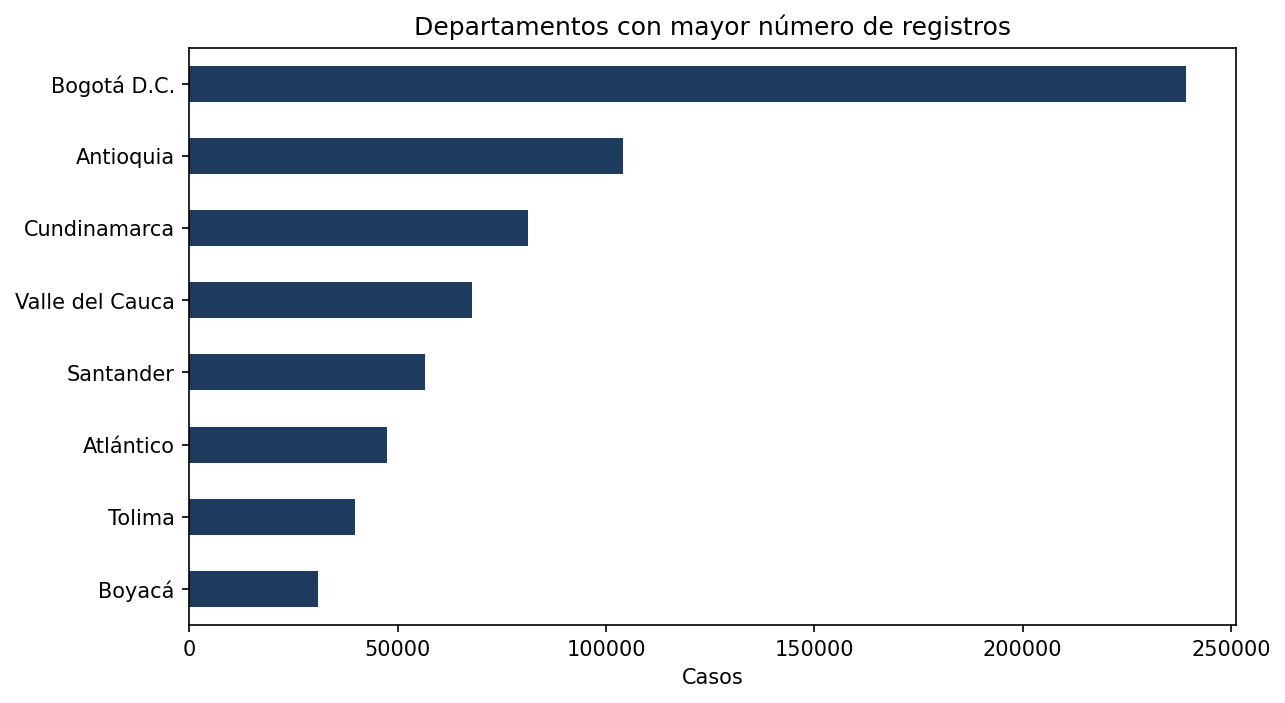
\includegraphics[width=0.92\linewidth]{figuras/02_top_departamentos.png}
	\caption{Departamentos con m\'as casos registrados. Elaboraci\'on propia con datos INMLCF \cite{medicinalegal2024}.}
	\label{fig:dept}
\end{figure}

Entre registros con zona informada, el 92{,}5\,\% del hecho ocurri\'o en cabecera municipal; el 4{,}6\,\% del total carece de dato de zona.

\subsection{Perfil de v\'ictimas y momento}

Hombres: 648.811 (66{,}1\,\%); mujeres: 332.800 (33{,}9\,\%).
Los grupos quinquenales (20--24) y (25--29) concentran 17{,}3\,\% y 16{,}7\,\%, respectivamente.
Domingo (180.420) y s\'abado (122.610) encabezan el conteo por d\'ia; las franjas 18:00--20:59, 15:00--17:59 y 21:00--23:59 concentran la mayor incidencia horaria.

\subsection{Configuraci\'on situacional}

Tras homologar v\'ia p\'ublica/calle, \emph{V\'ia p\'ublica o calle} re\'une 574.330 casos (58{,}5\,\%); le sigue \emph{Vivienda} (168.276; 17{,}1\,\%).
El mecanismo contundente aparece en 397.229 casos (40{,}5\,\%) y el mecanismo m\'ultiple en 243.615 (24{,}8\,\%).

La Figura~\ref{fig:sev} resume la severidad medicolegal seg\'un los intervalos INMLCF: 83{,}1\,\% en el rango \emph{1 a 30} d\'ias; 7{,}5\,\% sin incapacidad; 6{,}6\,\% entre 31 y 90 d\'ias; 2{,}7\,\% sin informaci\'on de incapacidad.

\begin{figure}[htbp]
	\centering
	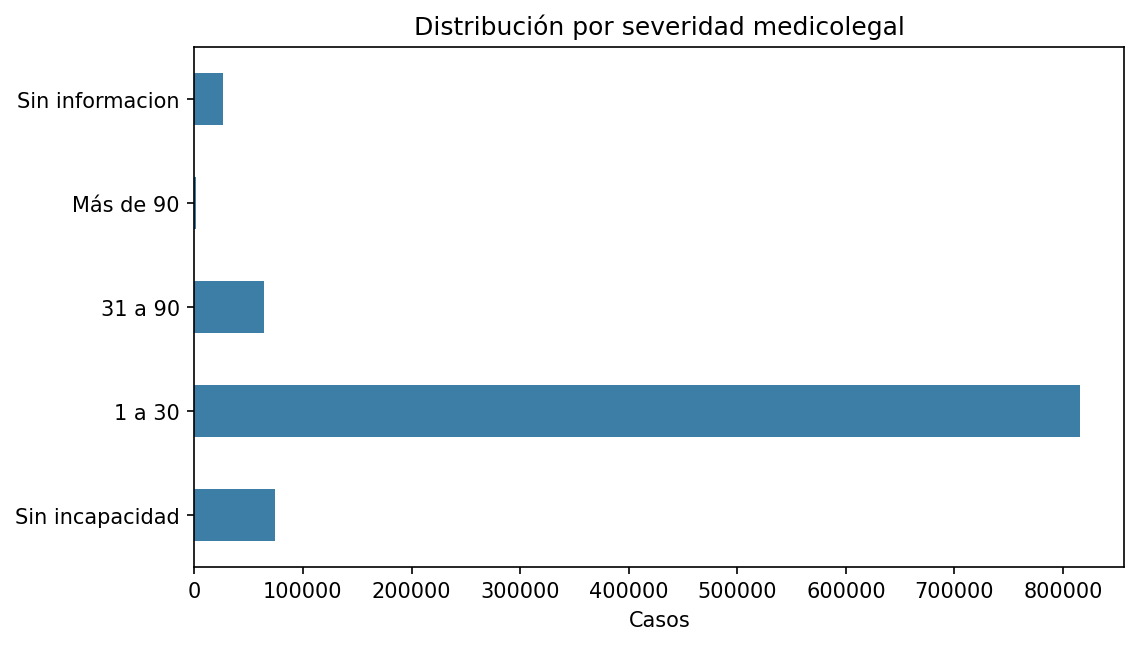
\includegraphics[width=0.92\linewidth]{figuras/03_severidad.png}
	\caption{Distribuci\'on por severidad medicolegal. Elaboraci\'on propia con datos INMLCF \cite{medicinalegal2024}.}
	\label{fig:sev}
\end{figure}

Entre presuntos agresores destacan \emph{Conocido sin ningun trato} (17{,}0\,\%), registro sin informaci\'on (16{,}8\,\%), \emph{Vecino} (13{,}7\,\%) y \emph{Polic\'ia} (10{,}6\,\%).

\section{Discusi\'on}

Los cuatro ejes permiten lectura integrada del fen\'omeno \emph{registrado}.
La ca\'ida de 2020 puede relacionarse con restricciones de movilidad y cambios en la demanda de valoraci\'on; no autoriza inferir reducci\'on real de violencia sin fuentes independientes.
La concentraci\'on en Bogot\'a D.C. y departamentos urbanos combina densidad poblacional, rutas de acceso a medicina legal y posible subregistro rural.

El predominio masculino y la edad joven-adulta, junto con escenarios de v\'ia p\'ublica y vivienda, apuntan a agresiones en contextos cotidianos de convivencia.
La codificaci\'on de incapacidad como intervalos categ\'oricos INMLCF (p.\,ej.\ \emph{1 a 30} d\'ias) no agota la gravedad cl\'inica o psicosocial del evento.

\textbf{Limitaciones.}
Subregistro y sesgo de denuncia; acceso desigual a valoraci\'on medicolegal; sensibilidad a cambios de protocolo; imposibilidad de inferencia causal; incapacidad codificada como intervalos categ\'oricos; homologaci\'on parcial de etiquetas INMLCF (v\'ia p\'ublica/calle, circunstancia y formato \emph{Amigo(a)} unificados; otras variantes permanecen separadas).

El dashboard facilita consulta y sustentaci\'on con filtros cruzados; no sustituye estimaciones poblacionales ni modelos predictivos.

\section{Conclusiones}

Se construy\'o un pipeline reproducible sobre 981.611 registros del INMLCF (2015--2024), con preprocesamiento documentado, cubo OLAP offline y dashboard Streamlit en cuatro ejes.
Los aportes son metodol\'ogicos y descriptivos: transparencia en la limpieza, agregados reutilizables y delimitaci\'on expl\'icita respecto de la violencia no registrada.
Extensiones razonables incluyen tasas por poblaci\'on, contraste con encuestas de victimizaci\'on y auditor\'ia de cambios en protocolos que expliquen rupturas temporales.

\printbibliography

\end{document}
